\documentclass[10pt,twocolumn]{article}

%%% packages %%%
\usepackage{color}
\usepackage{graphicx}
\usepackage{listings}
\usepackage{float}
\usepackage{url}
\usepackage{times}
\usepackage{xspace}
\usepackage{microtype}
\begin{document}

\title{SSA Construction and Optimization\ \\
  \small CSE 501 Spring 2013 Compilers Assignment 2}
\author{Andre Baixo, Jacob Nelson}
\maketitle

This writeup describes our optimizer implementation for Assignment 2.

\section{Implementation}

Our optimizer implements a number of optimizations. Here are the highlights:

\paragraph{SSA} 
We converted Start IL to SSA form using the algorithm described in
class, using dominance frontiers to place phi functions..

\paragraph{Constant Propagation} 
We implemented simple constant propagation.

\paragraph{Global Common Subexpression Elimination} 
We implemented Value Numbering.

\paragraph{Conversion from SSA} 
We use a naive approach, replacing phi functions with reads and writes
of temporary variables. We follow this with a pass that promotes most
SSA variables to registers in order to save instructions.

\paragraph{Code generation} 
We lay out code with a preorder traversal of the dominator tree for
each function. Care must be taken to update all branch targets and
function entry points.


Besides the generated code, our optimizer writes two forms of
debugging output. First, it dumps the all the requested information
about blocks, instructions, and dominators to a file. Second, it
writes the CFGs in GraphViz format. This may be converted to a
graphical representation using the \texttt{dot} program.

\section{Running}

The optimizer may be run by executing the \texttt{assignment2/run.sh}
script while inside the \texttt{assignment2} directory. We have
included precompiled intermediate languages files for all examples in
the distribution. Running the script will create separate output files
in the \texttt{examples} directory for each method of each example;
optimized intermediate language output has the extension
\texttt{.ilo}, dump information has the extension \texttt{.txt}, and
CFG output has the extension \texttt{.dot}. For example, the optimized
IL for \texttt{gdc.dart} can be found in
\texttt{examples/gcd.dart.ilo}. The GraphViz files can be turned into
PDF with a command like \texttt{dot -Tpdf file.dot > file.pdf}.

The script mostly follows the interface described in the assignment;
optimizations are selected by specifying a comma-separated list to the
\texttt{-opt=} flag, and similarily backends with the
\texttt{-backend=} flag. We write output to files as specified above
instead of stdout, since there is often a lot of output.

Our optimizer is implemented in Ruby, so no separate build step is
required. Ruby version 1.9 is required. 

\section{SSA discussion}

Conversion to SSA was reasonably stratightforward. We followed the
approach discussed in class; we computed dominance frontiers in order
to help us place phi functions. Then we used a collection of stacks to
rename variables.

Figure~\ref{fig:ssa-code} shows a simple test we used to debug our SSA
conversion. Figure~\ref{fig:pressa} shows the CFG before SSA
conversion, and Figure~\ref{fig:ssa} shows the CFG after SSA
conversion. This example requires only one phi function merging the
results of the four previous basic blocks; our phi functions have one
entry for each predecessor, even if values are duplicated. We can see
that the writes to the $x$ variable in the pre-SSA example are
replaced with writes to five different SSA variables, with a fifth
used to store the result of the phi function. We also see that the
read-only variable $y$ is not touched by the SSA algorithm, and its
initial value (denoted by a trailing \$ in our system) is used in the
write operation.

Figure~\ref{fig:postssa} shows the result of translating out of SSA in
our system. The phi function in this example is replaced by writes to
a temporary variable $\_\_x\$24$, which is allocated on the stack at
offset $-12$. This temporary variable is read in BB 19 in the
\texttt{write} instruction. Most of the intermediate SSA variables are
replaced with registers; note in particular that BB 13 now contains
only one memory write, instead of the three writes in SSA form.

Converting from SSA was a bit hairy. First, since we added and removed
instructions in the conversion, we had to renumber all instructions to
be contiguous so that the Start VM wouldn't complain. This required
fixing up all register operands, branch targets, and call
sites. Second, when promoting SSA memory operations to registers, we
had to fix up instructions that used the memory operations as
operands. We used a symbol table to track equivalences as we added and
removed instructions.

\begin{figure}
\begin{center}
  \begin{verbatim}

import 'stdio.dart';

void main()
{
  int x;
  int y;
  x = 0;

  if( 1 == 1 ) {
    if( 1 == 1 ) {
      x = x + 1;
      if( 1 == 1 ) {
        x = x + 1;
        x = x + 1;
        x = x + 1;
      }
    }
  }

  WriteLong(x);
  WriteLong(y);
  WriteLine();
}

\end{verbatim}
\begin{minipage}{0.95\columnwidth}
  \caption{\label{fig:ssa-code} Example program for SSA.}
\end{minipage}
\end{center}
\end{figure}



\begin{figure}
\begin{center}
  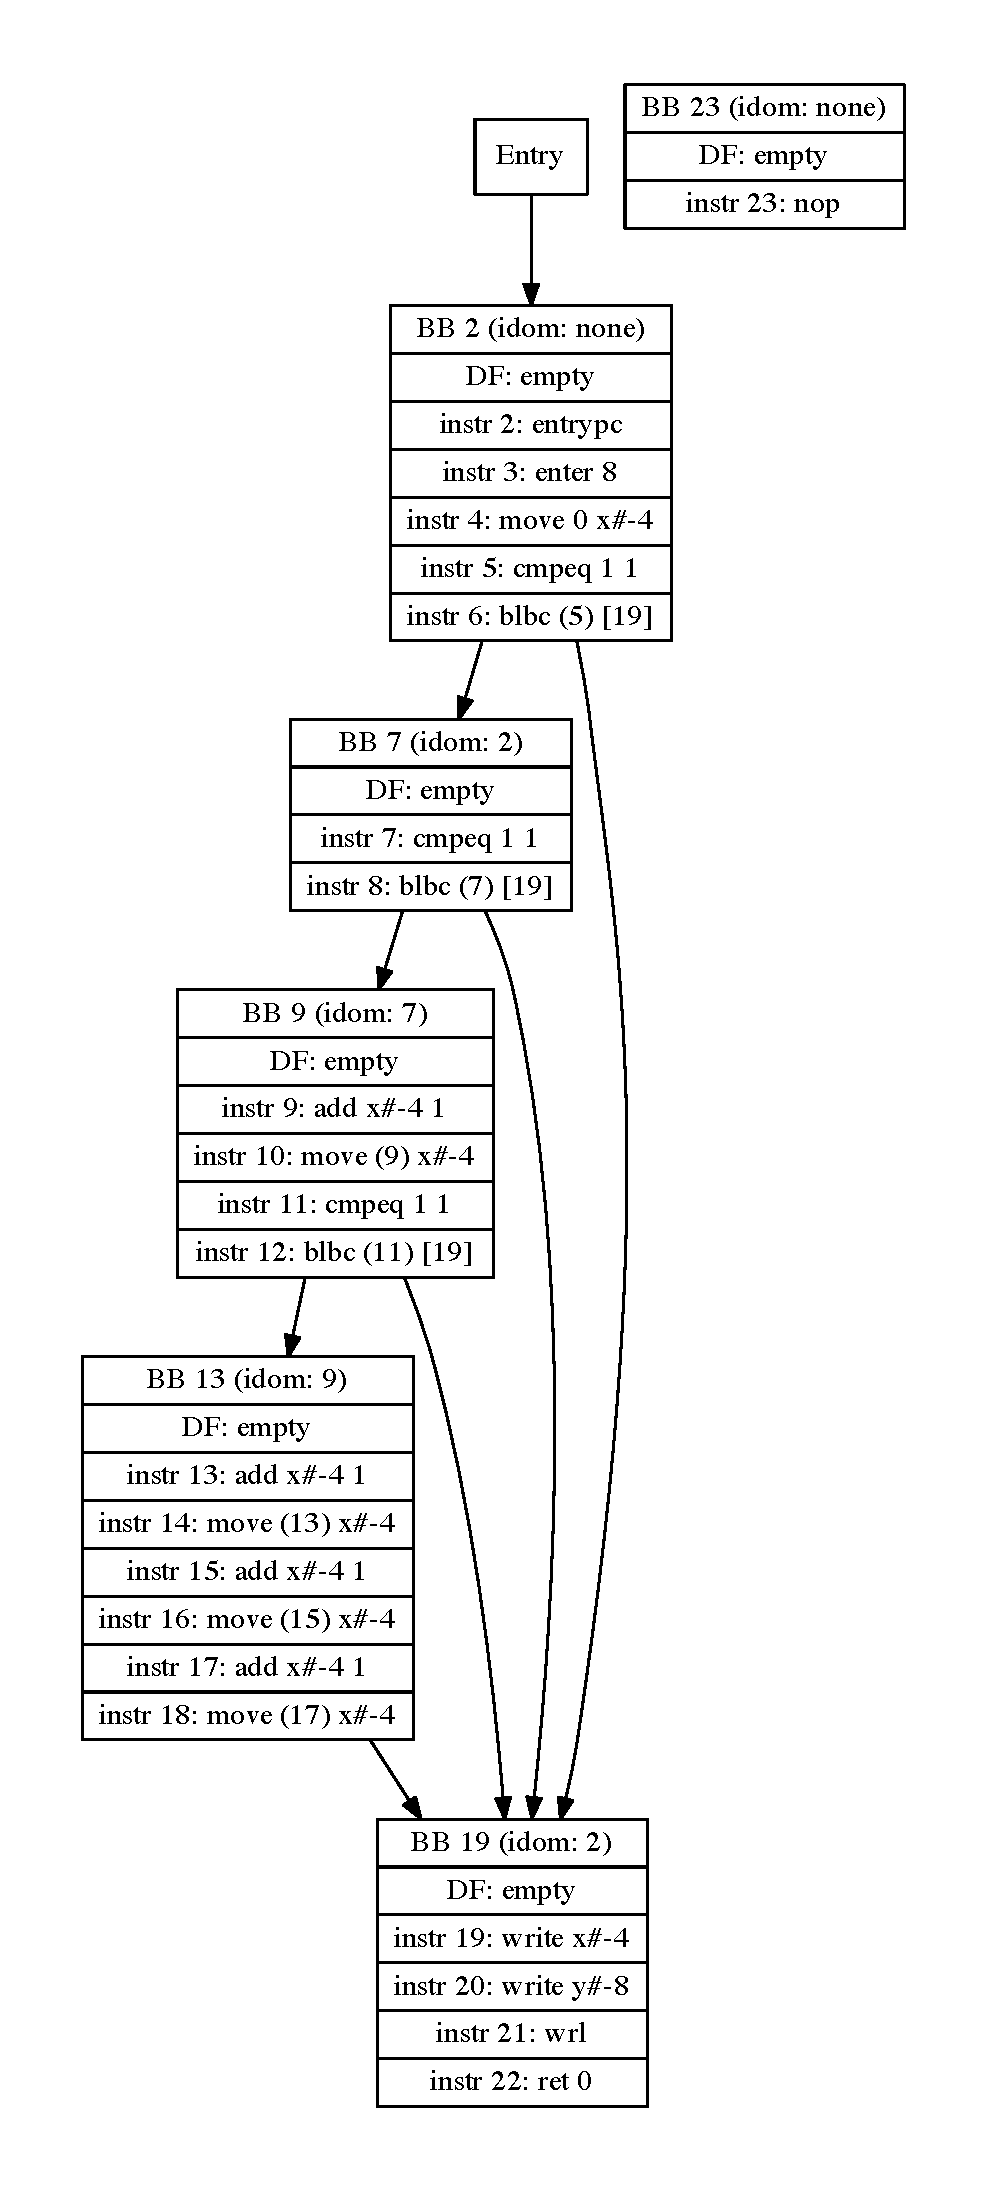
\includegraphics[width=0.95\columnwidth]{figs/simple6-pressa.pdf}
\begin{minipage}{0.95\columnwidth}
  \caption{\label{fig:pressa} CFG for Example~\ref{fig:ssa-code} before converting to SSA.}
\end{minipage}
\end{center}
\end{figure}

\begin{figure}
\begin{center}
  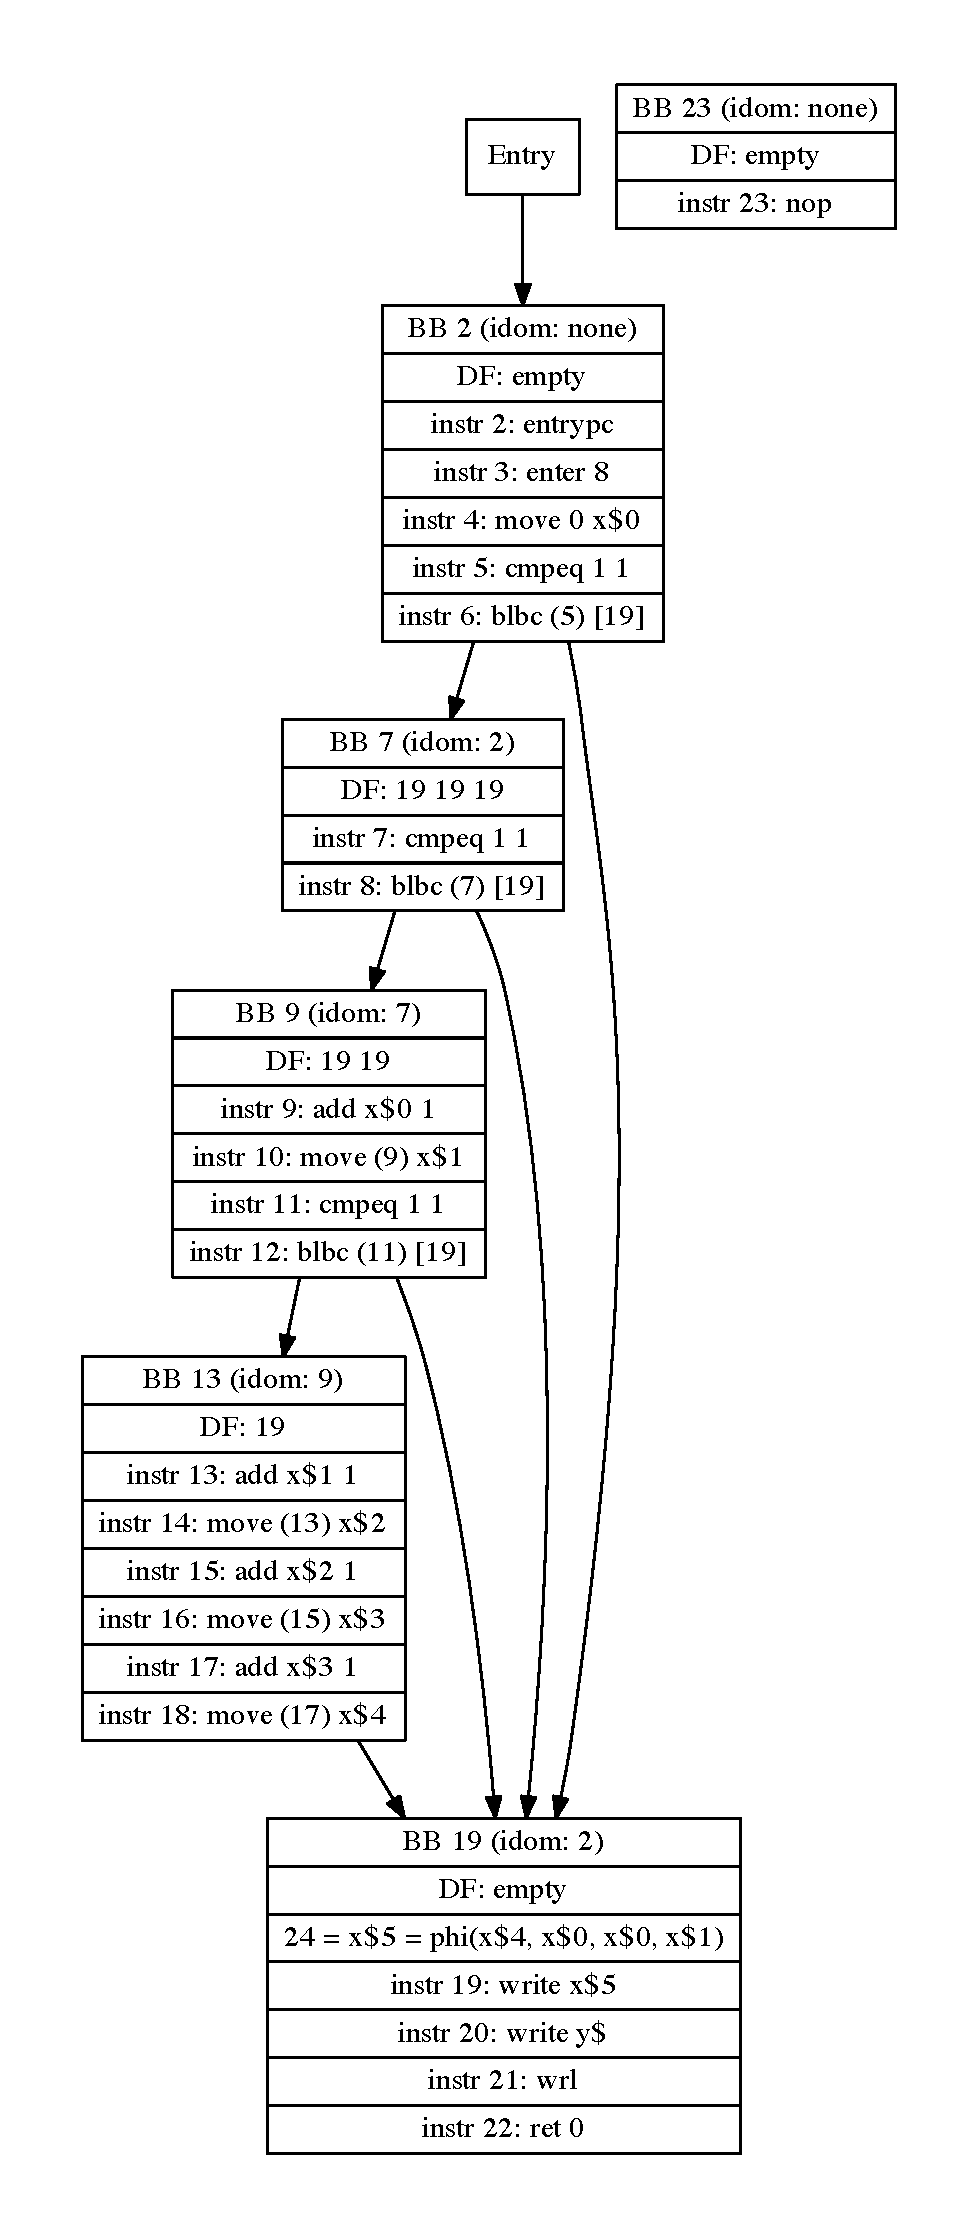
\includegraphics[width=0.95\columnwidth]{figs/simple6-ssa.pdf}
\begin{minipage}{0.95\columnwidth}
  \caption{\label{fig:ssa} CFG for Example~\ref{fig:ssa-code} in SSA form.}
\end{minipage}
\end{center}
\end{figure}

\begin{figure}
\begin{center}
  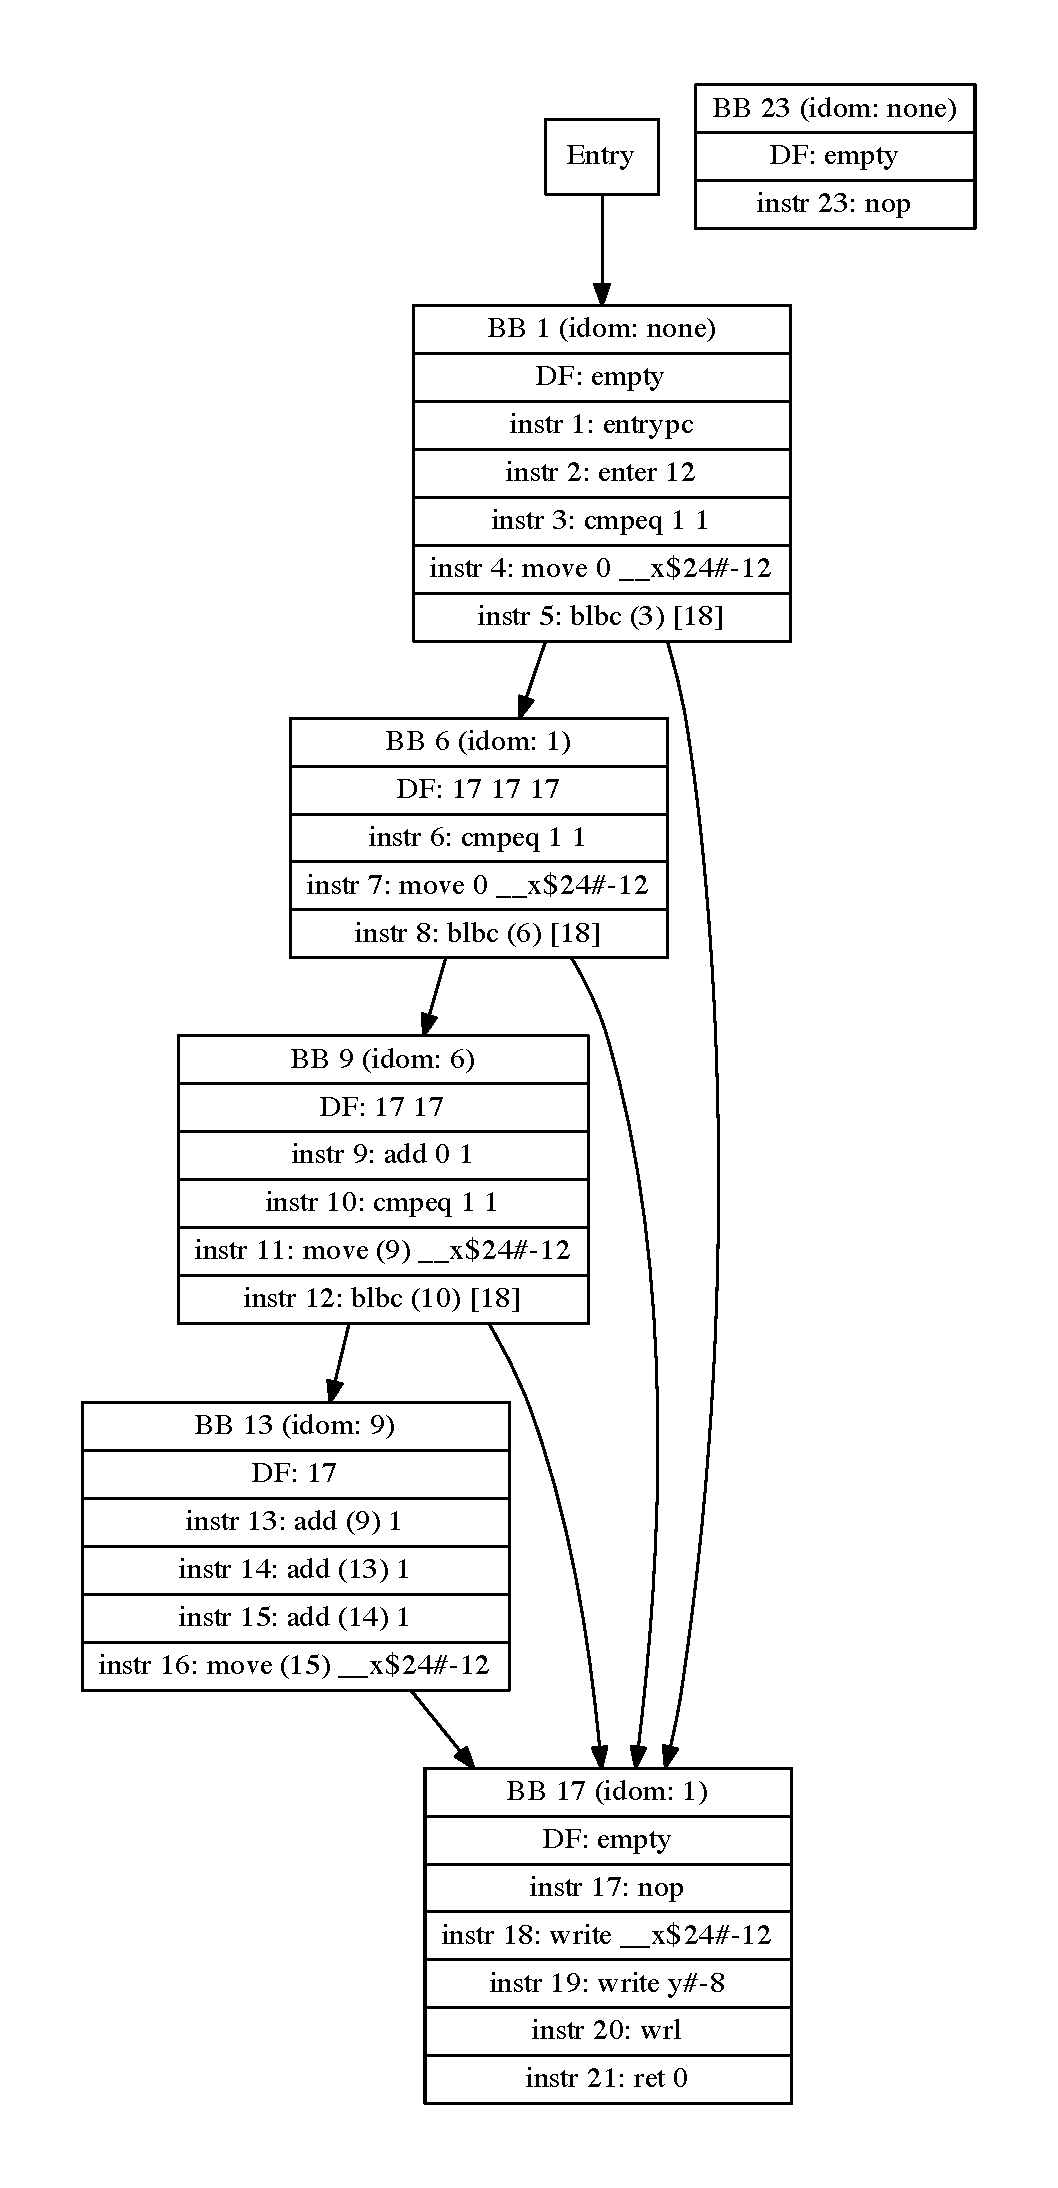
\includegraphics[width=0.95\columnwidth]{figs/simple6-postssa.pdf}
\begin{minipage}{0.95\columnwidth}
  \caption{\label{fig:postssa} CFG for Example~\ref{fig:ssa-code} after converting out of SSA.}
\end{minipage}
\end{center}
\end{figure}


\section{Constant propagation}

We implemented simple sparse constant propagation. We chose not to do
conditional constant propagation; neither did we remove dead code from
branches that were killed by constant
propagation. Figure~\ref{fig:postscp} shows how constant propagation
works for Example~\ref{fig:ssa-code}; we are able to eliminate all
computation from the example. 

\begin{figure}
\begin{center}
  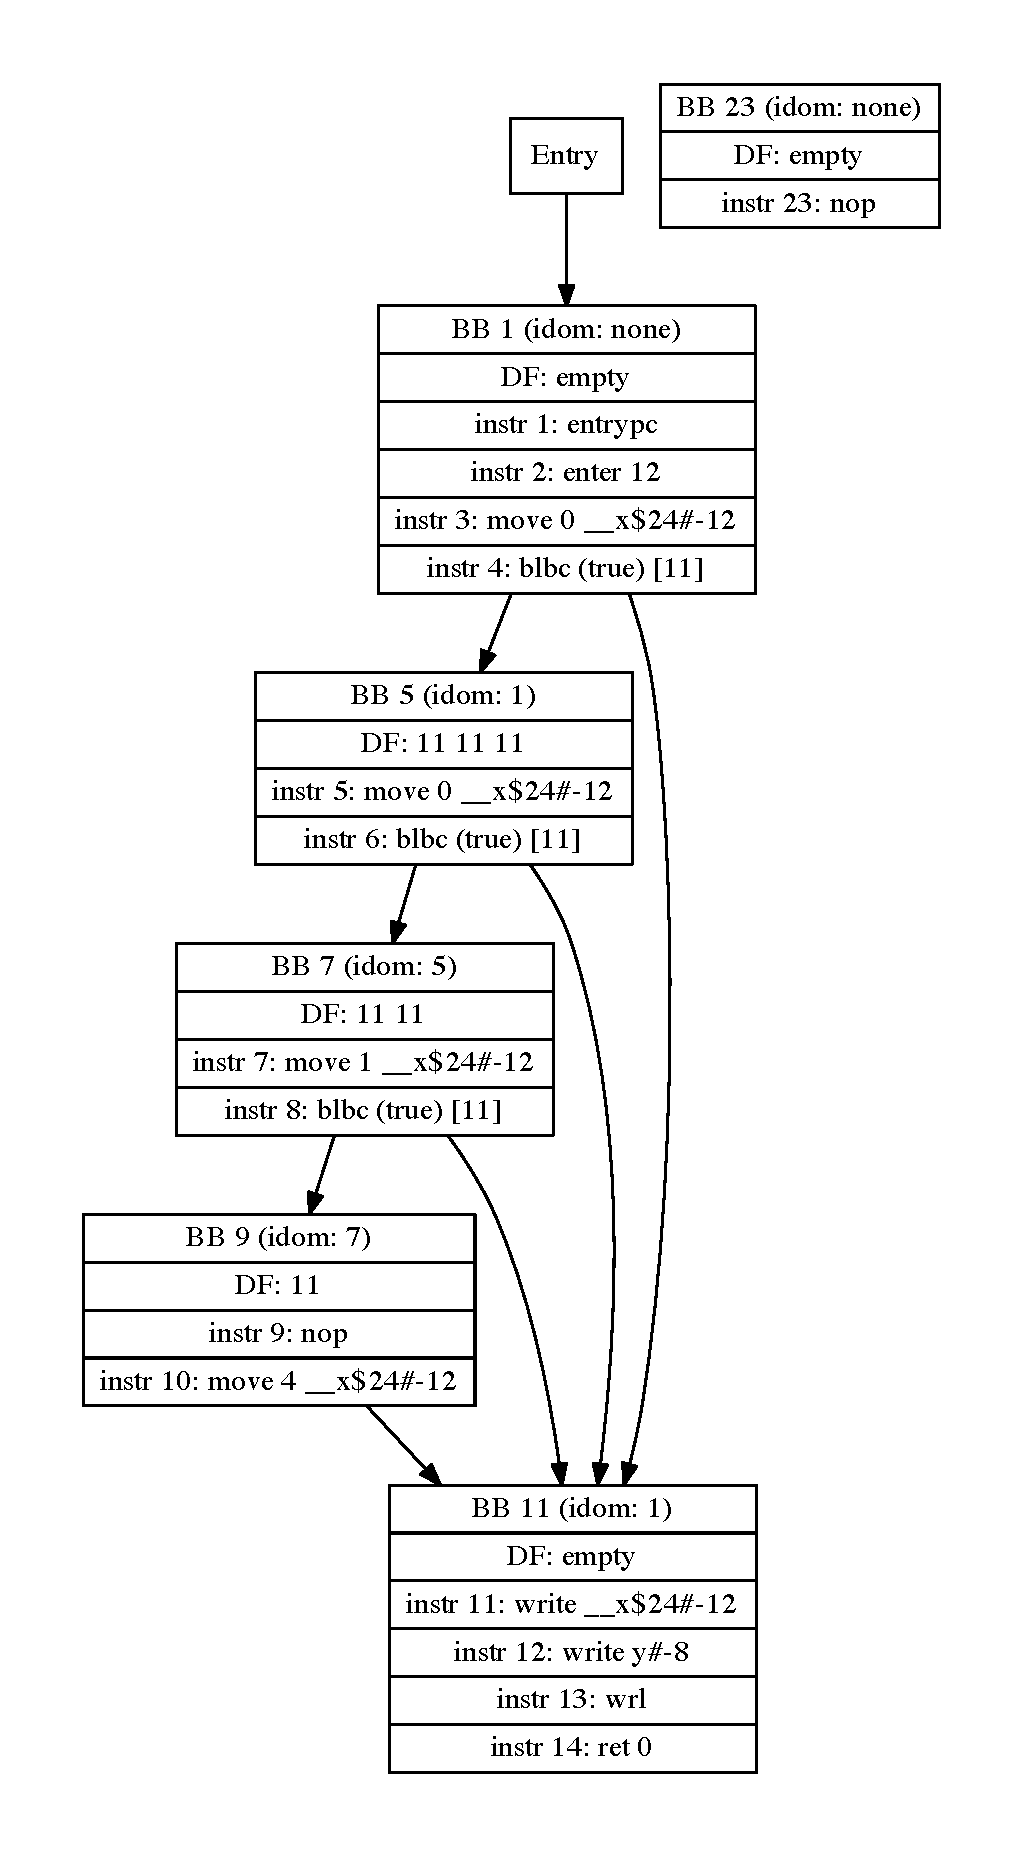
\includegraphics[width=0.95\columnwidth]{figs/postscp.pdf}
\begin{minipage}{0.95\columnwidth}
  \caption{\label{fig:postscp} Subset of CFG from \texttt{regslarge.dart} after applying constant propagation.}
\end{minipage}
\end{center}
\end{figure}

\section{Value numbering}

We implemented value numbering for a mostly-arithmetic subset of the
Start instruction set. Many of the other instructions had the
potential of performing complicated and perhapse side-effectful
operations in memory, and while we could possibly reason about
situations where optimizations could be safe we chose to keep things
simple.

%% \begin{figure}
%% \begin{center}
%%   \includegraphics[width=0.95\columnwidth]{figs/prevn.pdf}
%% \begin{minipage}{0.95\columnwidth}
%%   \caption{\label{fig:prevn} Subset of CFG from \texttt{regslarge.dart} before applying value numbering.}
%% \end{minipage}
%% \end{center}
%% \end{figure}

%% \begin{figure}
%% \begin{center}
%%   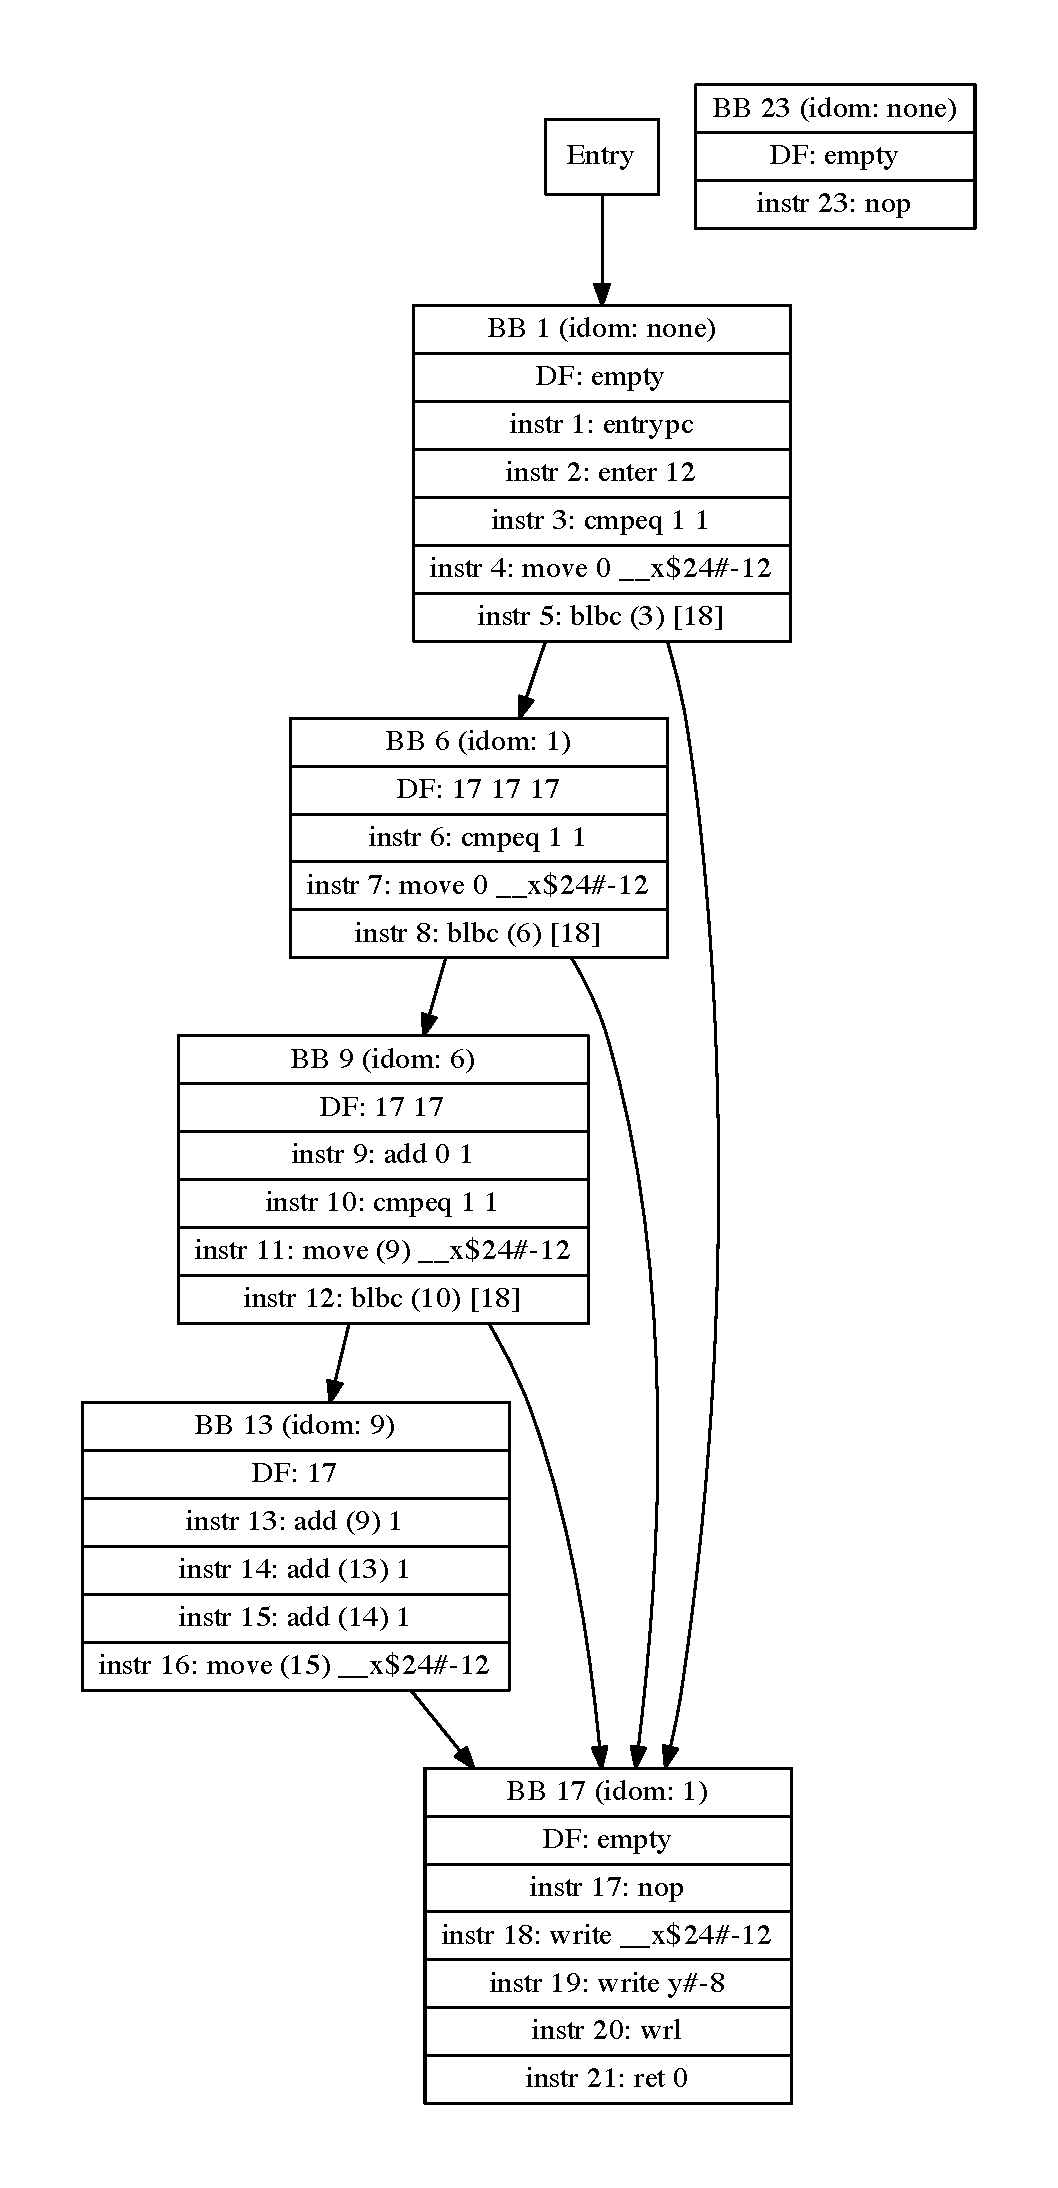
\includegraphics[width=0.95\columnwidth]{figs/simple6-postssa.pdf}
%% \begin{minipage}{0.95\columnwidth}
%%   \caption{\label{fig:postvn} Subset of CFG from \texttt{regslarge.dart} after applying value numbering.}
%% \end{minipage}
%% \end{center}
%% \end{figure}


\section{Conclusion}

We implemented a number of optimizations leveraging SSA representation.

\bibliographystyle{abbrv}
\bibliography{writeup}

\end{document}

